%% Hanford investigations

%% TCS schematic for LIGO Hanford for O3
%% TCS pre-loading
 %% Current methodology for tuning TCS
  %% Detail Hanford's methods
 %% Increasing RH tuning speed


As shown in Chapter 1,  increasing input power leads to a direct increase to the sensitivity of a DRFPMI to make gravitational wave detections. But one implication of this is the necessity for thermal compensation. As the interferometer increases input power, you directly couple more light into the Fabry-P\'{e}rot cavity arms; and even with optics ultra-low absorption ($\approx 400 \; \mathrm{ppb} \pm 150 \; \mathrm{ppb}$ \textcolor{red}{alog ? or point absorber paper}) still induce thermo-optic effects with the projected circulating arm power of 200 kW. A symptom of this is mode mismatch throughout the interferometer, a problem that contributes to loss of usable optical power throughought the DRFPMI which can reduce sensitivity two-fold: loss of power to your readout, and reduced efficacy of the current solution to reduce the quantum noise limit (squeezing).


\section{aLIGO Thermal Compensation System (TCS)}
Thermal deformations of mirrors can be superimposed, allowing an approximate restoration of the desired mirror radius of curvature with the usage of thermal actuators on the Fabry-Perot cavity mirrors at high power
\begin{itemize}
\item Annular actuation with RH actuators (Some notes about the analytical calculations of RH (There is a paper on this).

\item Central heating with central $\mathrm{CO}_2$ laser
\end{itemize}

\subsubsection{Wavefront sensing}
\textcolor{red}{Hartmann Wavefront Sensors}

\section{Mode Matching in O3}
Countering the problems that occur at high circulating power
requires estimated pre-load settings at higher power with the assumption that the test masses act as uniform absorbers.  The presence of high absorption points on the test masses (aka point absorbers) required adjustments to the TCS pre-load and various ring heater and CO2 settings were sampled. Part of this sampling lead to the development of a input ring heater filter allowing actuation to reach ? percent of the desired optical power within 2 hours compared to the 12 hour response pre-filter. Higher spatial frequency actuation in the form of a CO2 mask was also tried.

\subsection{Pre-loading for O3}
Reference to TVO's thesis for pre-loading settings based on his model \cite{tvo}

\subsubsection{Optimizing RH thermo-optic response}
With the inherent
\begin{figure}[H]
 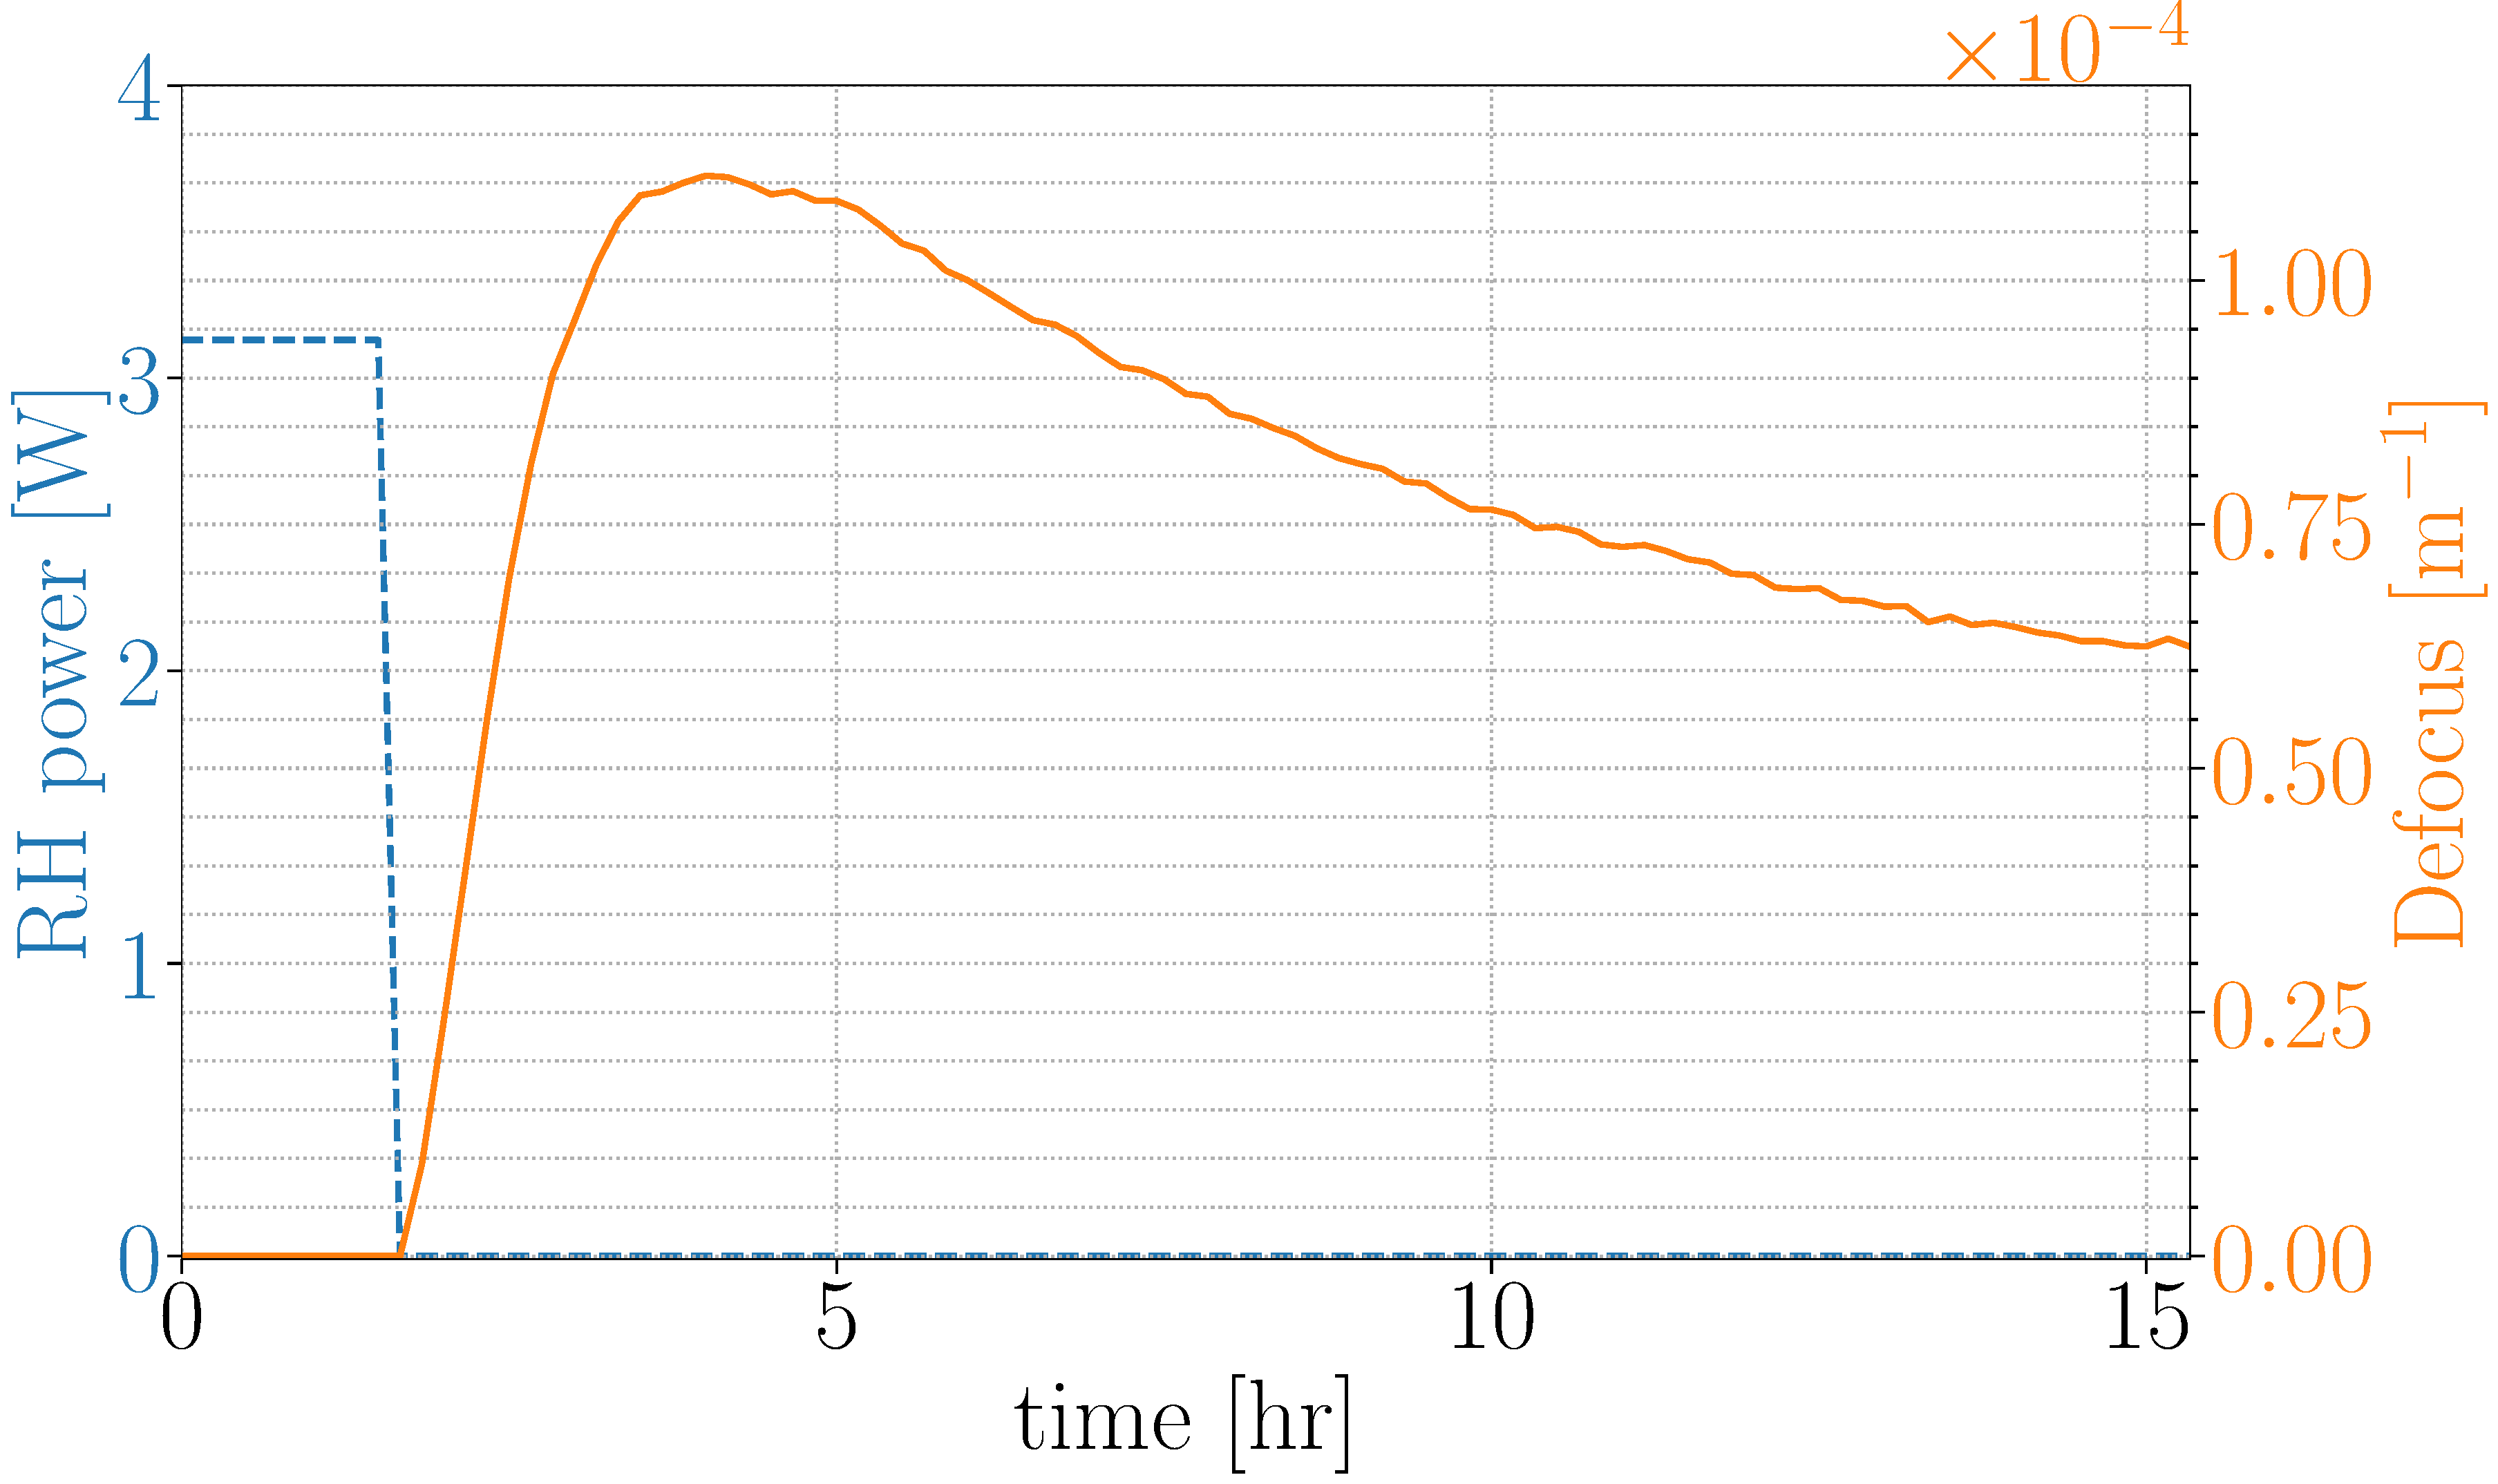
\includegraphics[width=\textwidth]{TCS/IRHF/Meas_response}
 \caption{ITMY thermo-optic response to a 3.13 Watt power reduction to ring heaters. It's after $\approx$ 12 hours after the change was made do you start to see a small enough $\frac{\mathrm{d} \alpha_\mathrm{sp}}{\mathrm{dt}}$ when you can assume a steady thermal lens.}
 \label{fig:meas}
\end{figure}

\begin{figure}[H]
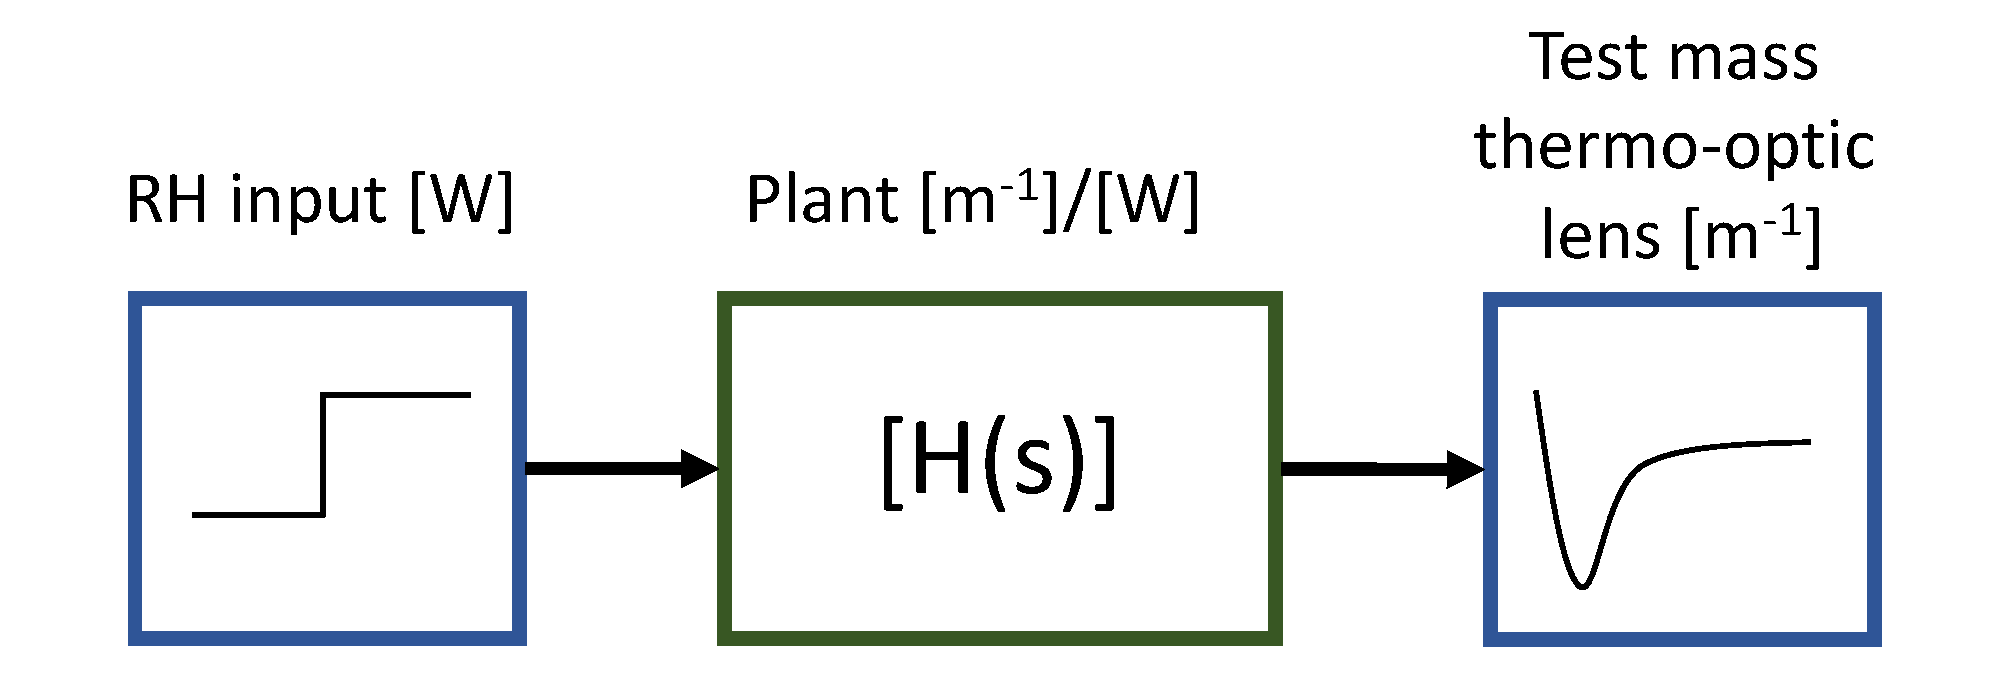
\includegraphics[page=1,width=\textwidth]{TCS/IRHF/RH_input_filter_figures.pdf}
\caption{A pictograph showing how the plant transforms the signal. The example of this can be seen in Fig [\ref{fig:meas}]}
\label{fig:justplant}
\end{figure}

\begin{figure}[H]
\includegraphics[page=2,width=\textwidth]{TCS/IRHF/RH_input_filter_figures.pdf}
\caption{A pictograph showing the system with real time digital filtering for an improved thermo-optic response. The RH input filter is created by inverting the plant filter combine with a low pass and added poles to the zpk model to ensure stability.}
\label{fig:plantwfilt}
\end{figure}

\begin{figure}[H]
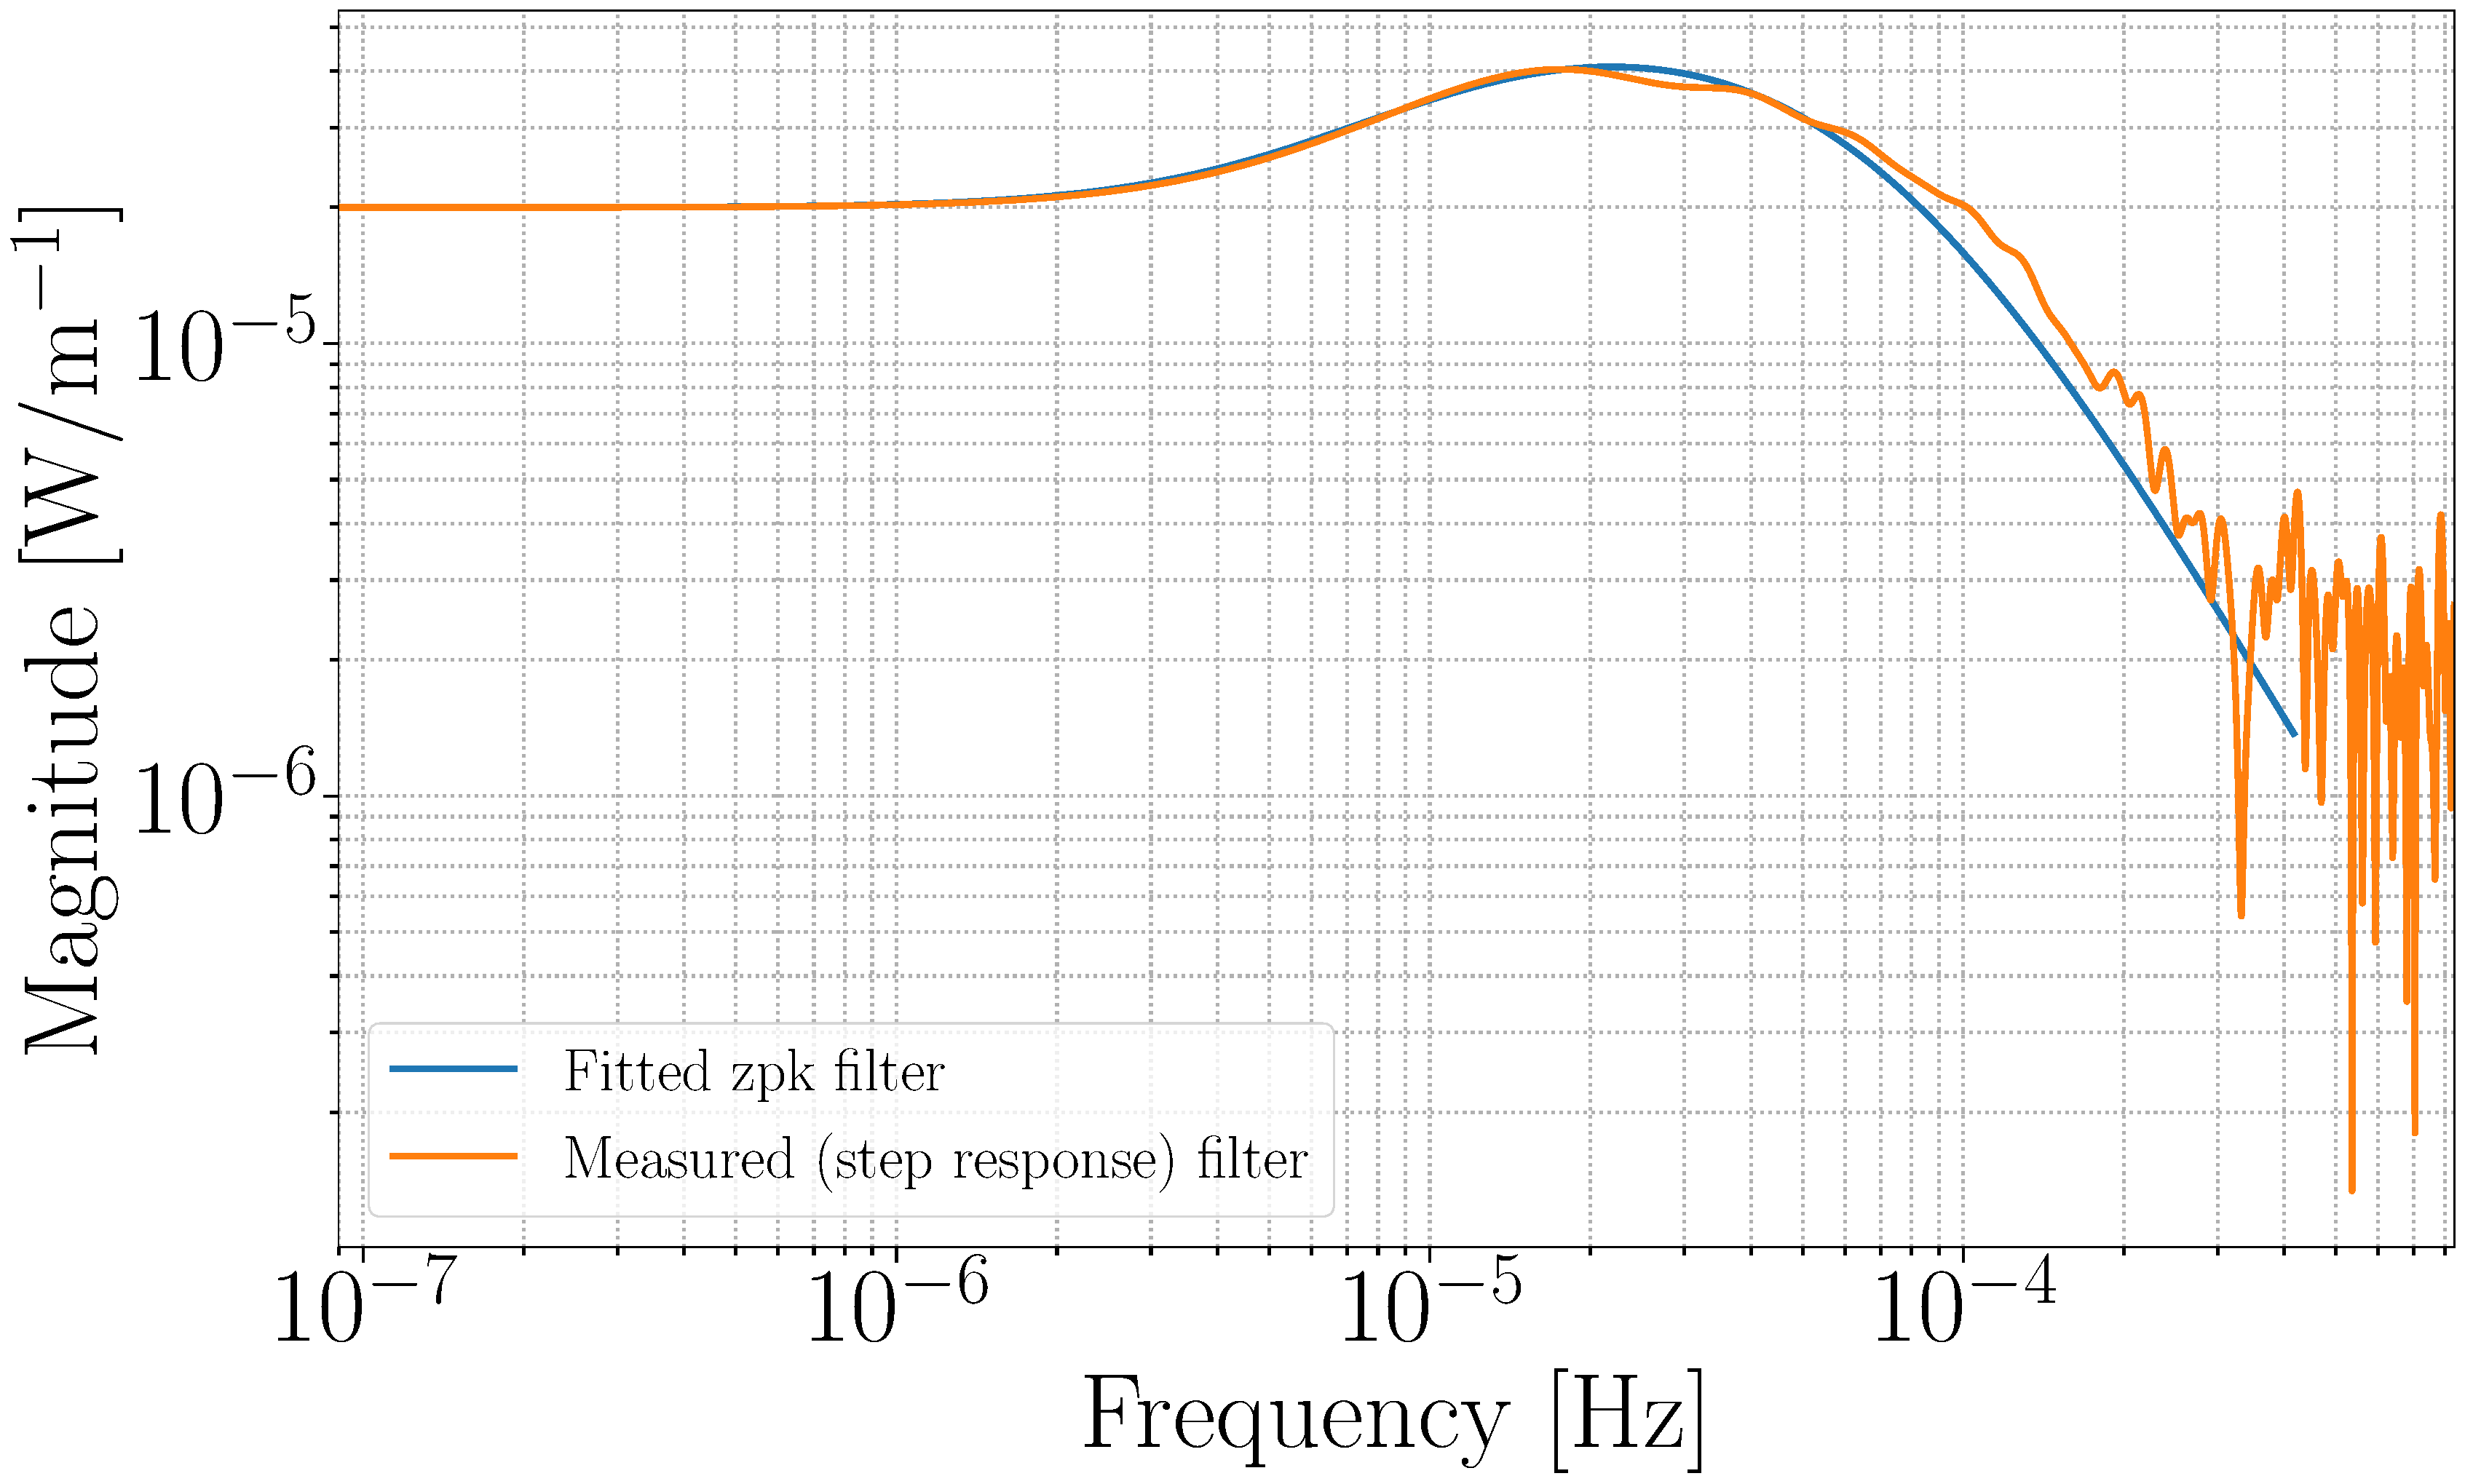
\includegraphics[width=\textwidth]{TCS/IRHF/RH_plant_filter_fit}
\caption{Showing the PSD of the RH response (normalized by the input RH power) over a an $\approx$ 12.5 hour period. The zpk model of the fitted filter (H(s)) is $9.2545e-12 \frac{(s+3.14210e-5)}{(s+8.168e-5)(s+0.0003142)(s+0.0005969)}$}
\label{fig:plant_v_fit}
\end{figure}

\subsubsection{Dynamic Thermal compensation}
\begin{figure}[H]
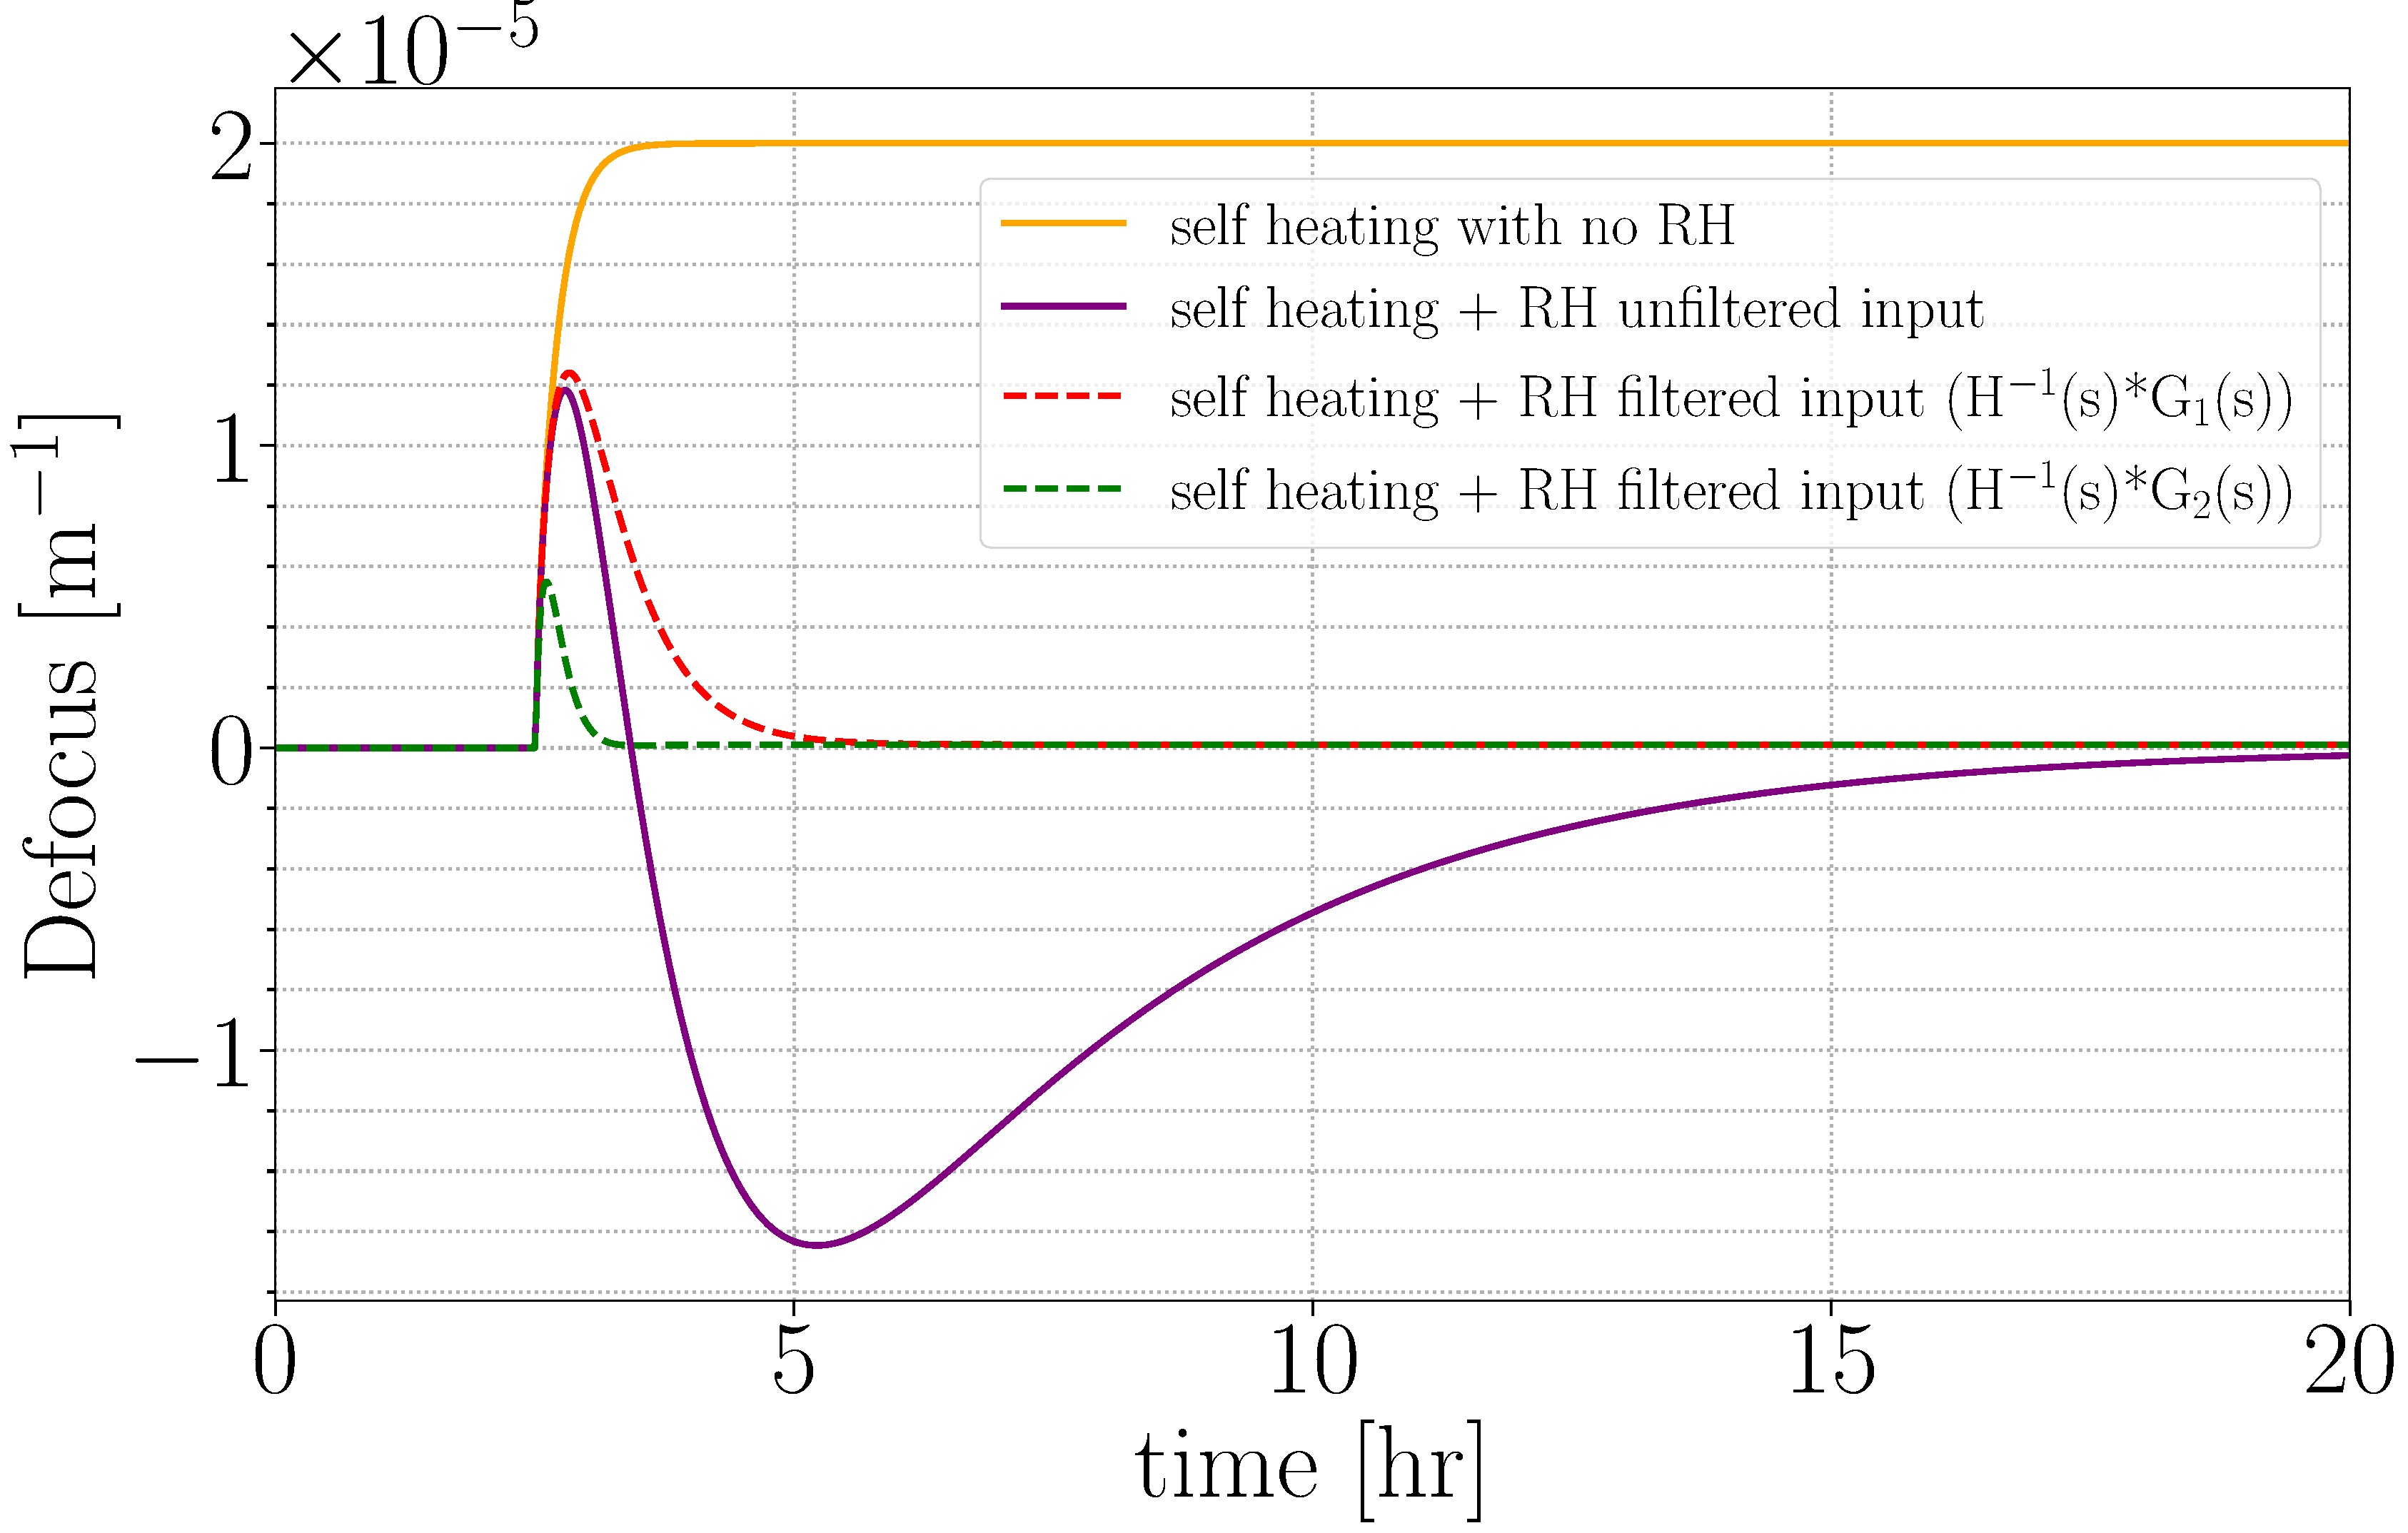
\includegraphics[width=\textwidth]{TCS/IRHF/IRHF_compare_w_self}
\caption{Comparison of the natural RH response and the response to the conditioned input. The above plot is simulated in Matlab by passing the RH input time series (top plot) through the $[H(s)]^{-1*}$ and $H(s)$ to acquire with the result lensing behavior on the bottom plot.}
\label{fig:dynam_comparison}
\end{figure}
\newpage


\subsubsection{Limitations}
\begin{figure}[H]
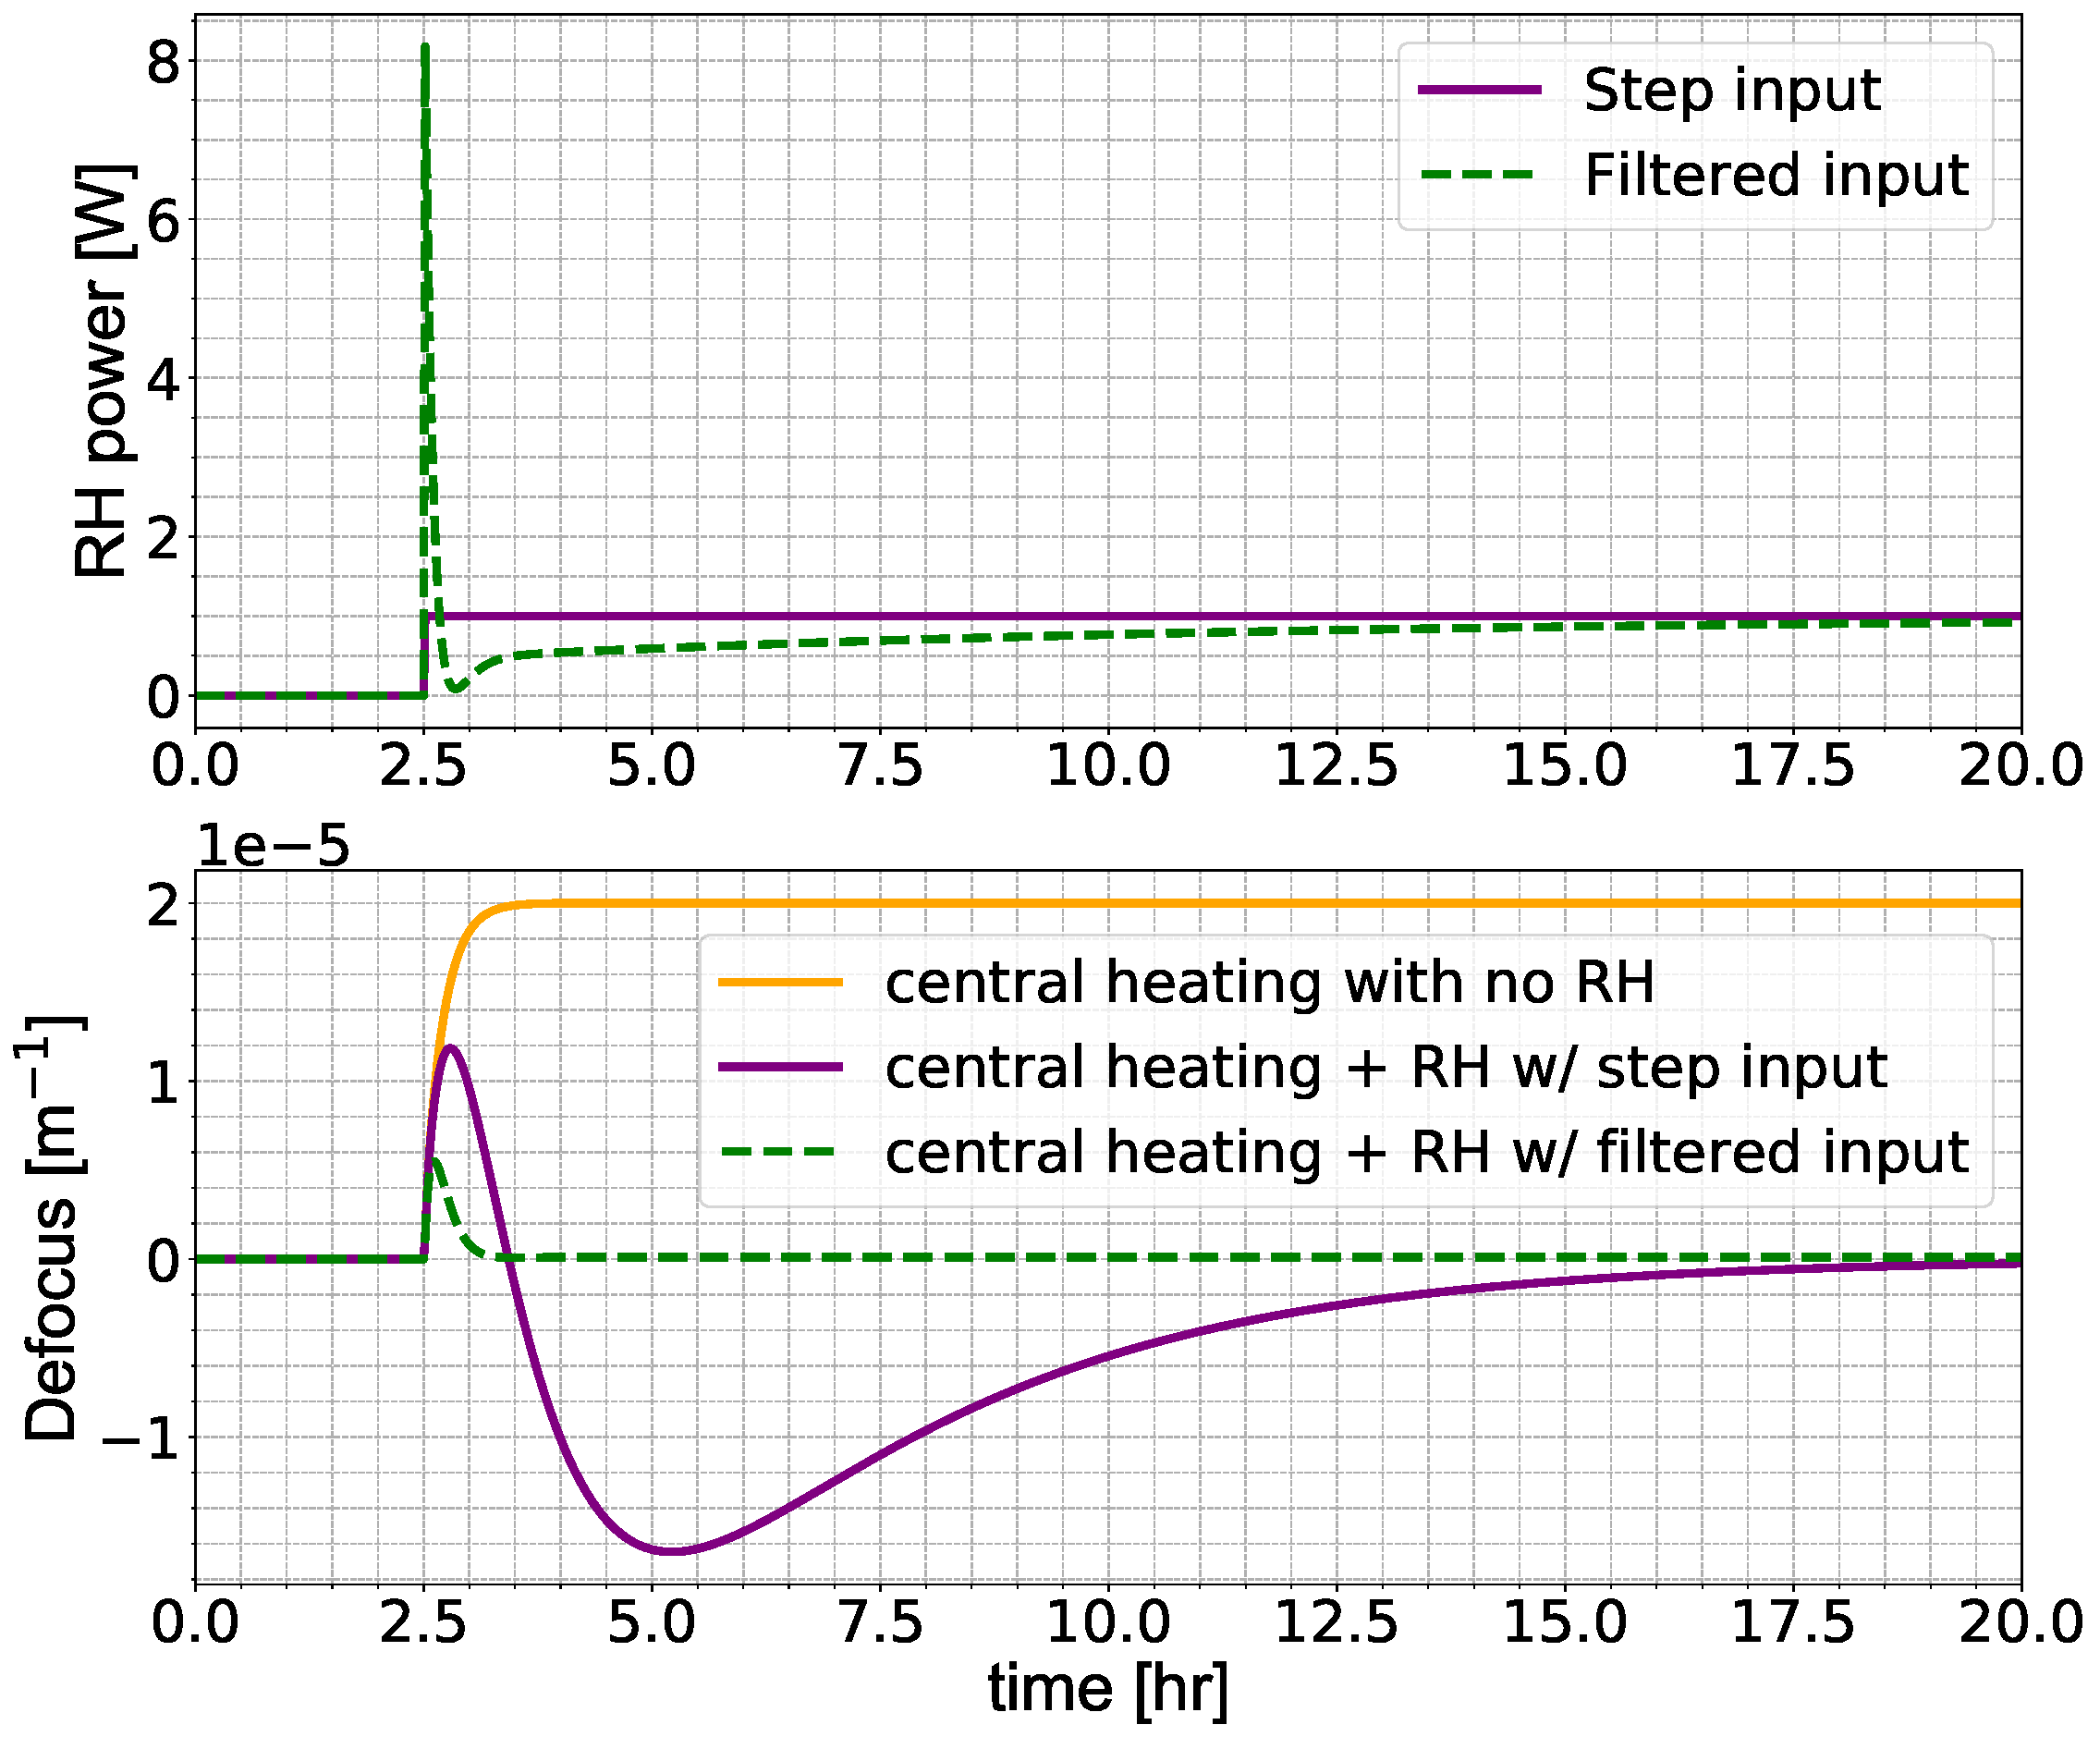
\includegraphics[width=\textwidth]{TCS/IRHF/IRHF_compare_w_RH_power}
\caption{Comparison of the natural RH response and the response to the filtered input with RH power}
\label{fig:RH_power}
\end{figure}
Limitation on RH power is set at 8W \textcolor{red}{Double check source?}

\textcolor{red}{Implementation into CDS at LHO (appendix?)}


\section{Higher order TCS}

\subsection{Point absorbers}

\begin{itemize}
\item Impact on RF sidebands with interferometer thermalization
\end{itemize}

\subsection{Actuation using a $\mathrm{CO_2}$ laser and mask}
\begin{itemize}
\item Aiden's design
\item Imaging
\item Installation
%\begin{figure}[H]
%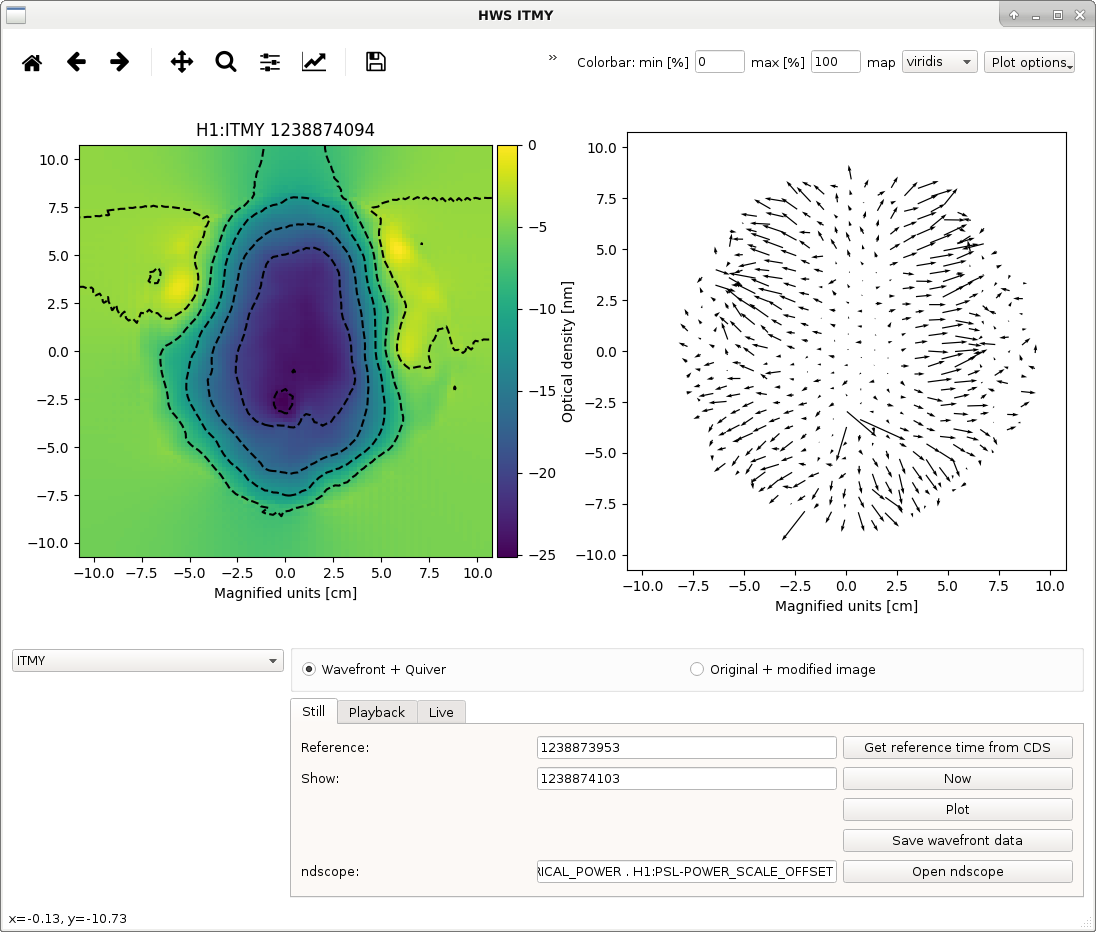
\includegraphics[width=\textwidth]{figs/TCS/PA/48349_20190409201649_inital_install_CO2Ymask2_150seconds_900mW.png}
%\caption{Point absorber figure with second $\mathrm{CO_2}$ mask}
%\label{fig:RH_power}
%\end{figure}

\item Metric of improvement? (Impact on sidebands after thermalization) (Tracking dither line amplitudes)
\end{itemize}
